\documentclass{project}
\usepackage[pdfauthor={Group 14},pdftitle={Software Engineering Group Project, Finl Report},pdftex]{hyperref}
\usepackage{color}
\usepackage{longtable}
\usepackage{graphicx}
\begin{document}
\title{Software Engineering Group Project}
\subtitle{Final Report}
\author{Group 14}     
\shorttitle{Final Report}
\version{2.0}
\status{Final}
\date{2014-02-16}
\configref{SE-14-FINAL}

\maketitle

\tableofcontents

\newpage

\section{INTRODUCTION}
\subsection{Purpose of this Document}
The purpose of this document is to give a view of the final 
state of the project. It will cover all aspects such as 
changes to the project plan that where made while coding and
Test tables to ensure the app worked as expected and
group reflection.

\subsection{Scope}
Everyone who wants a clear understanding of how the team functioned during this project should read this document. Individual members of the team looking for places that they could improve their teamwork skills may find suggestions in here as well.

\subsection{Objectives}
\begin{enumerate}
	\item Show changes made in the project over its lifecycle.
    \item Show how the project was collaborated on with reasons for the choices made
\end{enumerate}

\newpage

\section{MANAGEMENT SUMMARY}

The group achieved a working version of the Walking Tour Creator (WTC) that is capable of providing the user the means to record a walk and add a description about the walk, add points of interests at any point of the walk, also to be able to take pictures and have them saves and upload it to a database for viewing, in other words a fully functional personal Walking Tour Creator.
	
The group was able to verify that documents were in good state after the drafts had been reviewed. The majority of our documents got a grade of B and only one with a grade of C for the draft. The document with the C grade was in a bad state so what the group did was go and fix the issues with it to get the grade up. This dosn't mean that we left the other documents, they all had some minor issues so we delegated the fixes throughout the team to get them into a good state.

The group had minor issues with collaboration and version control. This was mainly due to group members struggling to use Git at the beginning of the project, so it was difficult to get all of the documents together. The way the group overcome these problems is that Dan Wakefield wrote a tutorial and put it on the repository. We also switched to using the free online \LaTeX{} editor \href{http://www.writelatex.com}{write\LaTeX{}} for producing documentation, as it allowed for easy collaboration (but consequently discouraged frequent commits to the repository).    

When developing the Android app, there was a major bug where if the user changed the orientation of their phone during an operation, the app would lose the asynchronous task, causing the task to attempt to open popups on an Activity that no longer existed. To overcome this, the Android sub-team passed the AsyncTask to a newly opened Activity each time this happened and updated the AsyncTask for the new Activity.

When developing the Web site, one of the problems that the Web sub-team had was deciding how to store in a database whether a coordinate was a point-of-interest or just an ordinary coordinate along the route. They overcame this problem by meeting together to work on it. They decided to add another column in the database which was a simple boolean value to represent whether a coordinate was a point-of-interest.

On a whole, the entire team performed with a hard-working attitude towards the goals of the project. While there were some issues with some group members not pulling their weight initially, by the end of the project each member displayed a passion and enthusiasm towards their work. Communication between the group was good particularly during integration and testing week where everyone showed a team spirit.


\newpage


\section{HISTORICAL ACCOUNT OF THE PROJECT}

At the begining of the group work, the group decided on major roles. These included Project Leader (Josh Tumath), Deputy Project Leader (Theo Taylor), QA Manager (Lars Lunde), Deputy QA Manager (Jake Maguire), Chief Architect (Rob Bolton) and Version Control Manager (Daniel Wakefield). Later during the prototyping phase of the project, the group was split into two development teams: the Android team and the Web team. These sub-teams were led by Rob Bolton and Jake Maguire, respectively.

The group met during Fridays for general meetings with the Project Manager. Additionally, there would be mid-week meetings, typically on Wednesdays, where the group would normally discuss the progress of work to be completed by the following Friday meeting. Facebook was the preferred platform for communication.

The first task the group had was to write the Project Plan document. This involved outlining what is to be produced and the architecture of both the app and website. This gave the group a first attempt at working together to produce something. Each section was given to different group member to work on. If a section required more work compared to others, more group members were be assigned to it.

Following this, the group was tasked with two documents to produce simultaneously. These were the Test Specification and the Design Specification. During this time, many members of the group had other assignments. Fortunately, the test Specification did not require too much time to write. Therefore, only Dan Wakefield was tasked to write it. The Deputy Project Leader led the creation of the Design specification with James Mellors and Michel Oddie. They delegated sections of the Design specification to each other. James Mellors was assigned to do the dependency description, Theo Taylor was assigned to do the introduction, decomposition description and the interface description, and Michel Oddie was assigned to do the detailed design.

Before the submission of each of these documents, a formal review meeting would be held by the Project Leader and QA Manager. Following this, issues would be created on GitHub listing the necessary changes.

During the creation of the Design Specification, the members of the group who were not working on it were simultaneously producing the prototypes for Android application, the front-end of the Web site and the database. This ensured every member of the group had work while also allowing for efficiency in the rate at which work was completed. By Christmas, both the Android sub-team and Web site sub-team were able to give a good demonstration of the front-ends of their software to the Project Manager.

Following the Christmas break, integration and testing week itself was a very busy week because of the great amount of work that needed to be completed in time for the Acceptance Test with the Project Manager at Friday afternoon. The way the group tackled it was to begin with a meeting together to talk about how far along we are and what tasks need to be done. The group made a plan of what needed to be done for each day. After the meeting, the group looked for a suitable workspace to allow them to work together.

Once the group was set up, they separated into the two sub-teams; as was the case during the prototyping stage. The sub-team leaders then delegated all the tasks that needed to be completed for the day. This process of meetings and task delegation was repeated each day of integration and testing week and the group found it to be a very efficient way of handling the work load.

Towards the end of the week, the app and Web site were coming together. This meant that some group members had no tasks assigned to them and therefore worked on revisions of previously submitted documentation to be efficient with their time.

During the Acceptance Test, the Project Manager was pleased that the majority of the produced software was fully functional. 


\newpage


\section{FINAL STATE OF THE PROJECT}
\subsection{Android App}

\subsubsection{Features}
The features of the app were mostly correct. The only feature that was missing was the ability to edit previous
Points Of Interest.
Most features were implemented correctly, except that the app is meant to tell you if you try to take a Point Of Interest
without any GPS signal, and prevent a Point Of Interest from being created. Instead, our app uses the user's last know location
for the new Point Of Interest.
GPS, the UI, and server interaction all work correctly.

\subsubsection{User Interface}
The UI works correctly. The user cannot any invalid data and are told what is wrong when they attempt to do so.
The user cannot navigate to displays which would not make sense e.g. returning to the "Create a new walk" Activity
whilst a current walk is being created.
The UI can properly handle the user pressing the home button or rotating the screen on certain windows. These are
any which require input before closing, and cannot be dismissed. Any windows which can be dismissed will not return
upon the user opening the app again.


\subsubsection{GPS}
The GPS collects data correctly and filters any points which are not accurate enough. The only issue
with the GPS is that it will automatically use the last known position if no new data is available, after
warning the user once that they need GPS data.


\subsubsection{Points Of Interest}
The only issue with the Points Of Interest is that the they were meant to have "one or more" images, but we allowed the
user to have no images as well.
The user can take as many pictures as they want, and when adding pictures to a Point Of Interest, they can look through thumbnails
of pictures they've already taken. Tapping on a picture deletes it. This was our interpretation of editing a Point Of Interest.

\subsubsection{Server Interaction}
Aside from a memory issue, the server interaction works well. It attempts to upload the image to the server and if anything
other than an http "200 OK" is received then the user is told that their upload failed. The user can attempt to upload again
if they want. This means that if anything goes wrong with sending the image then the user will be told - this includes website
issues and connection issues.


\subsection{Website}
\subsubsection{Features}
All features work correctly. The only potential issue would be if two separately uploaded images had the same hash. If this
were to occur then the old image would be overriden with the new one.
Parsing of the uploaded JSON and saving this data in the database works correctly.

\subsubsection{Walk List}
The page which displays the list of all recorded walks works correctly, and they are shown in a large grid with the walk's
name and a picture from it.
If a walk has no image then the app/webiste logo is displayed instead.


\subsubsection{Walk Viewer}
The walk viewer works correctly. On the left of the page it gives the user the walk's name, short \& long descriptsions, the total distance covered, how long the walk took. On the right the walk is displayed using Google Maps. Walks are correctly displayed in this area, with each GPS point and Point Of Interest being linked.

\subsection{Documentation}
%TODO: Add issues with documentation here


\newpage


\section{TEAM MEMBER PERFORMANCE}
\subsection{Josh Tumath (jmt14) - Project Leader}
Josh was given the role of Project Leader, where he led and directed the team in preparation for the final implementation of the software. During integration and testing week, he was also a Web Developer in the Web site sub-team, due to his previous experience in Web programming and design.

It was remarked by other project members that Josh was very well-organised throughout the duration of the project, planning the team's actions well. He was generally very helpful towards others; being easy to work with and not forceful in regards to pushing for completion of work.

However, Josh could be very unclear about deadlines, failing to set targets for when particular sections of work should be completed. Additionally, he did not delegate work evenly, leaving some members to be completing more work than others.

\emph{The above report was agreed to by all members of the group.}


\subsection{Theo Taylor (tht5) - Deputy Project Leader}
Theo was given the role of Deputy Project Leader, where he led group meetings in times when the Project Leader was unavailable. He also led ad-hoc sub-teams that worked on a specific task for the project, such as the Design Specification. He was also an Android Developer in the Android sub-team.

During integration and testing week, Theo worked on certain features in the Android app, such as disabling the back button and creating Bundles for communication between Activities. He struggled in this area due to a lack of experience with Android development.

However, overall Theo could be quite unreliable at times. Additionally, when leading members of the team, he failed to push for high quality of work - being too lenient towards slacking and meeting deadlines. For example, the Design Specification required many last-minute changes before it was handed in.

\emph{The above report was agreed to by the group member.}


\newpage


\subsection{Lars Lunde (lah25) - QA Manager}
Lars was given the role of QA Manager, where he took minutes in meetings, held formal reviews and aided the group in meeting the QA standards.

As Lars's native language is not English, he was concerned this may affect some of the duties of his role. However, this was not an issue. For the most part, he followed through with his role effectively, and was willing to put in the hours for the sake of the group. During integration and testing week, he was very focused and worked closely with Rob on the development of the Android app, while always ensuring he had work to do.

The main issue with Lars was that he could be very slow at publishing meeting minutes - usually taking more than 24 hours after the meeting. Additionally, as the weeks progressed, his minutes became less detailed, which affected some members’ understanding of their tasks following the meetings, or reminding themselves of the items discussed during the meetings. Furthermore, he did not enforce the Java coding standards during integration and testing week.

\emph{The above report was agreed to by the group member.}


\subsection{Jake Maguire (jam64) - Deputy QA Manager}
Jake was given the role of Deputy QA Manager, where he mainly took minutes in meetings when Lars was no able to, and prepared formal reviews when the QA Manager was too busy. During the prototyping and implementation stages of the project, he was also tasked as Lead Developer of the Web site sub-team, due to his previous experience in server-side programming. Additionally, he allowed us to use his Web server for hosting the Web site.

From the beginning of the project, Jake had been very helpful and involved. When taking the minutes for meetings, he would usually be very prompt in uploading them. He also worked hard on developing the user interface design of both the Android app and the Web site. Jake had very good attendance of meetings and in the computer rooms during implementation and testing week.

Jake had proven himself to be very efficient in leading the Web site sub-team, as the majority of their prototyping and final implementation has been completed by Christmas. However, it is possible that he took on more work himself and not enough for group member James Berry.

\emph{The above report was agreed to by the group member.}


\subsection{James Berry (jab73)}
James was given the role of Web Developer in the Web site sub-team, where he aiding in the early prototyping and implementation of both the client-side and server-side systems. This suited James's skillset, having studied Web development in previous university modules.

James was reliable in both attendance and completion of work. At the beginning of the project, he wrote the risk analysis and a schema for the Tour database, which were done to a high standard. Working with Jake Maguire, they worked efficiently to complete a prototype of the Web site before Christmas.

During integration and testing week, James put a lot of work into researching how to solve certain problems, such as decoding base64 encoded images on the server-side. Additionally, he aided with the Google Maps APIs to ensure the front-end was feature-complete. Finally, James was very helpful in competing the PHPdoc.

\emph{The above report was agreed to by the group member.}


\subsection{Rob Bolton (rab26)}
Rob was given the role of Chief Architect, where he was expected to handle the overall design of the system from initial planning to implementation. In early meetings during the project, he expressed an interest and ability in planning class structures and imagining relationships between parts of the system. During the prototyping and implementation stages of the project, he was also tasked as Lead Developer of the Android sub-team. This required him to gain a detailed understanding in in the Android SDK - building on his experience in using the Java programming language.

Rob displayed a great passion for the work of the project and a strong desire for work to be completed to a high standard. He explained that he has enjoyed the experience; particularly during integration and testing week, when he stated that he thrived from the pressures of working towards a deadline and being heavily relied upon by other members of the team. He was also very helpful and patient with other Android developers in the team when allocating and expecting work from them.

However, he was perhaps too willing to take on too much work for himself. Much of the work on prototyping for the Android app was completed by him - as was much of the coding for the completed app. One night, he and Dan Wakefield stayed awake for over 24 hours to work on the final features for the app.

\emph{The above report was agreed to by the group member.}


\newpage


\subsection{James Mellors (jam66)}
James was given the role of Android Developer in the Android sub-team, where he helped with smaller changes in the development of the Android app. However, James's more significant contributions were towards documentation efforts, where he worked on various sections of the Project Plan and Design Specification. In addition, he designed the logo of the software.

James very quickly proved himself to be reliable and prompt when the project began. Work he was given - such as gathering information on the Google Maps APIs or writing about the high-level architecture of the Android app - was completed promptly. He was always seeking or work to do.

During the former half of integration and testing week, James did some peer programming on adding certain features to the Android app, such as checking if a device supports location services. In the latter half, he worked on the UI and updating the design specification.

\emph{The above report was agreed to by the group member.}


\subsection{Michael Oddie (meo9)}
Oddie was given the role of Android Developer in the Android sub-team, where he aided in the implementation of the Android app. However, he was initially tasked to create the initial wireframe design for the Web site and certain sections of the Design Specification. During integration and testing week, he worked mainly on testing and documentation.

Initially, Oddie's meeting attendance and contribution effort could be quite poor. Part of this was due to society events clashing with the group's unofficial weekly meetings. Other times, however, work was simply not being completed or completed late - namely specific sections of the Project Plan he was tasked on completing. This improved over time, and, by the latter half of Semester 1, he was contributing much more.

Oddie performed greatly during integration and testing week, when he was very enthusiastic about working on the Android app and testing it very extensively. This showed he thrives much better in a constant working environment. He was a great value to the team, working with other members of the group to help them and ensure that they were producing a good quality of work.

\emph{The above report was agreed to by the group member.}


\newpage


\subsection{Dan Wakefield (daw46)}
Dan was given the role of Version Control Manager, where he acted as a consultant for the group when using the project repository on GitHub. This required him to attend a lecture on the subject and maintain the health of the tree during development. He also aided in the development of both the Android app and the Web site.

Though Dan lacked access to an internet connection off-campus during Semester 1, he still put in a great deal of work and contribution towards the project. Over the course of the project, Dan’s experience with Git improved greatly, and his help was invaluable by integration and testing week. 

He worked very hard on the project. Most notably, he devoted a lot of time to helping Jake Maguire and James Berry to fix a critical bug in the communication between the Android app and Web server. At one point, he stayed awake overnight with Rob Bolton trying to refactor the software when the completion of some features was behind schedule.

\emph{The above report was agreed to by the group member.}


\newpage


\section{CRITICAL EVALUATION}
In terms of final product, the whole team performed efficiently and competently. The project was finished on time with nearly all the functionality that was specified at the start. Our initial designs were thorough to the point where the implementation of the project did not encounter errors or big changes from what we decided early on.

Each member played their part in the project with everyone coming together at the end to get everything done. The Project Leader made sure that progress was being made in the appropriate places, that all team members had a job to do and that deadlines were set to ensure the project would be finished on time. Everyone pulled their weight and was commited to getting their part done for the rest of the team.

There were a few issues with delegation with those in various leadership roles preferring to tackle most things on their own rather than delegating tasks to other member on their team. With more organised delegating the project may have been completed quicker and a rush at the end to get everything completed would have been avoided.

Communication could have been better in terms of responding promptly to questions and tasks on online platfroms such as GitHub and Facebook. It could be hard getting a response from all members quickly when a question was asked or tasks assigned on GitHub would be left open even if completed.

Improvements could have been made during our project lifecycle. Git was an under-utilised tool by some members, especially by the Web team. Due to a lack of knowledge, complications with merges and branches were apparent during implementation. This led to Git being side-lined and meant features such as rolling back to previous versions and allowing multiple members to work on the same file could not be used effectively.

Our project also had some missing functionality. The ability to edit locations on a walk was not present, which was reflected in our acceptance testing. This was more a oversight from the team rather than a technical issue, but meant that our Android app did not do everything that was asked by the Requirements Specification. 

The team learned about the importance of communication and how critical it is to keep in contact to track progress and know what to do. The minutes had to be taken with detail so that members who were unable to attend the meeting still knew what task they would have to complete that week. Both the Web sub-team and Android sub-team leaders had to communicate to make sure that things were set up at their own ends to allow tests to take place between the two platfroms, to check they were interacting with eachother corectly. The Project Leader had to communicate tasks to each member giving them specific targets of deadlines and the content of their work. Feedback from members would also have to be given to the Project Leader in terms of whether or not these targets were attainable or if they had disagreements with what had been set.

Another lesson learned was the equal importance of all stages of the project life cycle. Our emphasis on a proficient design meant that our implementation ran into little problem and allowed us to finish on time. The analysis we carried out early on meant that most functionality was in place as we knew what was required from our end programs, making our project a viable solution to the specification given to us at the start.

\newpage

\section{APPENDIX A: PROJECT TEST REPORT}
\subsection{TEST TABLE}

\begin{longtable}{ | p{2cm} | p{1.5cm} |} 

\hline 
{\bf Test Ref} & {\bf Result} \endhead  \hline

SE-F-001 
& PASS \\ \hline

SE-F-002
& PASS\\ \hline

SE-F-003 
& PASS\\ \hline

SE-F-004
& PASS\\ \hline

SE-F-005
& PASS\\ \hline

SE-F-006
& PASS\\ \hline

SE-F-007
& PASS\\ \hline

SE-F-008
& PASS\\ \hline

SE-F-009
& PASS\\ \hline

SE-F-010
& PASS \\ \hline

SE-F-011
& PASS\\ \hline

SE-F-012
& PASS\\ \hline

SE-F-013 
& PASS\\ \hline

SE-F-014
& PASS\\ \hline

SE-F-015
& PASS\\ \hline

SE-F-016
& PASS\\ \hline

SE-F-017
& PASS\\ \hline

SE-W-001
& PASS\\ \hline

SE-W-002 
& PASS\\ \hline

SE-W-003
& PASS \\ \hline

SE-W-004
& PASS\\ \hline

\end{longtable}

\newpage

\section{APPENDIX B: MAINTENANCE MANUAL}

\subsection{Walking Tour Creator}
\subsubsection{Program Description}
This application allows a user to record a walk, tracking their GPS coordinates and allowing them to add named points of interest with pictures. It can upload this walk to a server once it is finished.

\subsubsection{Program Structure}
The component diagram can be found in \textit{Design Specification 3.1.1}
The sequence diagram can be found in \textit{Design Specification 5.1}
A list and definition of the classes \& interfaces and their methods used can be found in the Design Specification:
\begin{itemize}
\item \textbf{MainAppActivity} \textit{4.1}
%TODO: Finish this once design spec is more finished
\end{itemize}

\subsubsection{Algorithms}
The significant algorithms can be found in \textit{Design Specification 5.2}

\subsubsection{Main data areas}
The main data areas can be found in \textit{Design Specification 5.3}

\subsubsection{Files}
Our application does not use any specific files. The only files it relies on being there are the photos taken for the Points Of Interest.
The path returned by the camera intent after taking the photo is used for these.
If the application cannot find the file, then the photo will not be added to the JSON before sending it to the server.

\subsubsection{Interfaces}
The only requirements for the application to successfully function are that the user has a camera, internet connection, and GPS running.
If the user does not have a camera then they cannot install the application.
If the user does not have GPS running then the application will not let them create a new walk. Turning this off whilst the application is running
will prevent the application from gaining any more GPS data, and it will continue to use the last know location for new Points Of Interest.
If the user does not have an internet connection then saving and uploading the walk to the server will fail.

\subsubsection{Suggestions for improvements}
Several improvements could be made to the application. At the moment there is no way to edit points of interest after they have been created.
In order to fix this, I would recommend having a new activity using a list view and an adapter, which takes the Walk in its bundle to see
which points of interest we have.

When the methods converting the walk to JSON were created they were made as a quick solution to upload the walk.
As a result of this they attempt to compile the whole walk in one go. This means that the entire JSON object of the walk is in
memory. Two solutions which would help are downscaling the image before converting it to base 64, and finishing the code which
converts and sends the JSON one image at a time in a stream. Realistically, both of these should be completed for good practice, as we do
not need high resolution images on the website, and storing the whole JSON object in memory can cause phones with small amounts of memory
to crash.

\subsubsection{Things to watch for when making changes}
There are a couple of places in which you need to take care when changing. Anything dealing with an AsyncTask needs to ensure that if it displays any dialogs
that the context it originally had is still available for use. An example of doing this correctly is where we call "setDialogsAndNotify" on our walkUploader
in order to give it the new dialogs for the current Activity.
Another area in which it is important to take care when changing is the JsonPackager. Any changes to the format of the JSON in here need to be reflected
in the website's code which deals with the received JSON.

\subsubsection{Physical limitations of the program}
There are a few physical limitations of the program.
In order to be able to install it, the user's device needs to have a camera.
If the user does not have GPS when attempting to create a new walk then they will be not be able to create one.
If the user does not have enough memory to store all of the images they took, then the application will crash upon
compiling the JSON representation of the walk.
Another physical limitation is that the application will not accept any GPS data which is too inaccurate. This uses the Location.getAccuracy() method
and filters out any results which are greater than 15 meters. This method returns \textit{accuracy} in meters, which is a circle of radius \textit{accuracy}
which has a 68\% probability that the device was within the bounds of this circle.
Due to this, if the device never receives any Location objects which are at least within 15 meters accurate then no GPS data will be recorded.
The last limitation is that the user needs an internet connection to upload the walk. The application will keep the walk until the user successfully uploads
it or cancels it.

\subsubsection{Rebuilding and Testing}
All of the documentation is either in LaTeX or Javadoc. Any pdf\-to\-LaTeX compiler should work for rebuilding any of the LaTeX documentation.
The Javadoc can be rebuilt using Eclipse by selecting \textit{File \-> Export... \-> Java \-> Javadoc} and following through with the wizard.
Another alternative is to use the "javadoc" command.

\newpage

\subsection{Walking Tour Displayer}

\subsubsection{Program description}
This Web site receives tours from the Walking Tour Creator and stores the data within a MySQL database. Web site visitors can view a list of the tours and view each of them on a detailed map that displays the route with points-of-interest along it.

\subsubsection{Program structure}
A list of significant functions can be found at \textit{Design Specification 2.2.2} and a component diagram can be found at \textit{Design Specification 3.1.2}

\subsubsection{Algorithms}
The significant algorithms can be found in \textit{Design Specification 5.2}

\subsubsection{Main data areas}
The main data areas can be found in \textit{JSON QA 2.1}, \textit{2.2}

\subsubsection{Files}
There are two main files that the walking tour displayer relies on. The first being the css file for the website, which is stored in the directory /projects/wtc/css and is responsible for the layout of the website. The second directory being /projects/wtc/images which contains all of the images for the webpage. This directory also includes another subdirectory called /images/walkimages, which is where all of the images sent from the app are stored.

\subsubsection{Interfaces}
The walking tour displayer has been tested on many different browsers, including mobile devices. On mobile devices the user is unable to scroll on a marker if there are many different pictures. The only browser that the website has not been tested on is IE6 so the user may encounter problems on that particular browser.


\subsubsection{Suggestions for improvements}
You could entertain the idea of adding a search bar to the website. This would be particularly useful when the website is populated with a large amount of  walks. You could add a search bar where the user can serach for a particular name of a walk that they wish to view. An SQL statement would then be used to search through the database and return the results of the search. Ajax could be used to create a more dynamic webpage, where the results for the search would get returned while a user is still typing in there search. Other search features that could be implemented would be to search walks by the distance or by the time they take to complete.

  Another feature that could be added is to print out the directions for the walk next to the map. I imagine that there is probably a google api which can be used to do this automatically, which would save quite a bit of time. This api would check all of the  coordinates and guide the user through their walk, giving them directions for the turnings that they need to take.

  A pagenation should also be considered where large amounts of data are being used so that the user would not have to endlessly scroll through all of the walks, but rather go through pages with a certain amount of walks per page. This could be implemented using a php script which takes in all of the walks from the database and then divides them all by a certain number, say 9, and splits all of the walks into several pages of 9 walks.

  A final feature that should be added to the website is to have a clear start and a finish of the walk. At the moment the map only displays all of the coordinates and locations of a walk, but it is not clear where the walks start and end. The only clue is that the centre of the map is set to the first coordinate. However this can cause confusion, partiularly if the walk is a giant loop which start and finishes in the same place. To overcome this a marker, similar to those used for a location but different in some way, should be used to show where the fisrt coordinate is and the last coordinate is.
  
\subsubsection{Things to watch for when making changes}
It should be noted that if you wish to change any of the SQL querying, we have used a PDO abstraction layer to implement these, rather than using the MySQLi APIs.

\subsubsection{Physical limitations}
As our Website has been written on a personal server, it should be noted that if it is intended for this website to handle a greater amount of traffic then it would be necessary to move to a new host server, as the current server only allows for a certain amount. There is also a limit to the disk space available, so if there is expected to be a large amount of data stored on the server, particularly with image data, then extra disk space will most likely be needed to stop this from becoming a problem.

\subsubsection{Rebuilding and Testing}
As this has been written on a personal server, the files cannot be easily viewed. However they are all avalable at "www.jakemaguire.co.uk/projects/wtc".

In terms of testing the website, the best thing to do would be to run the app and put some dummy data in, including some locations with pictures to see that they write correctly to the database and then check the website homepage to see that it then displayed correctly.

\newpage

\section{APPENDIX C: REVISED PROJECT PLAN}

\section{OVERVIEW OF PROPOSED SYSTEM}

\subsection{Project Overview}
Our app that we are going to produce will be android based.
Our app is going to be a walking tour app that will help people make their own 
walks and to be able to edit and save them to view again a later day.

Platforms to be used and Architecture for the app:
gskip

\subsubsection{Android}
The assignment stated that we have to make an app for android 
phones so thats the platform we will be using, as well as using android platform version 2.2

\subsubsection{PHP}
We will be using PHP for the website and for the phone to communicate 
to the server (database). I think we will find it easier to use than 
javascript and it will be a good opportunity to get better at writing 
in that language. We plan to host the Website on our group member Jake Maguire's personal VPS and the web address for the project will be www.jakemaguire.co.uk/projects/wtc

\subsubsection{JAVA}
Java is what we will be using to program the app. We just need to
decide what we will use to write it in, there is a choice between
eclipse with the android plug in or android studio. Our preference will be to use android studio

\subsubsection{MySQL}
MySQL is what we will be using to make the database to be able 
to store the walks that have been created. 

\subsection{High Level Architecture}
\subsubsection{Map API}
The map will be a big part of our app because we will need to display the
routes and be able to let people see where there going and make their own
route. We will be using the map api on our web server to display a selected route from the database.

\subsubsection{App UI}
The Menu / UI, first we will have the main page where you will 
be able to click on the button create new route to be able to start mapping 
the path while you are walking, right underneath this button their will be 
2 more preferences and exit. All together there will be up to 4 menus to 
this app: main page, naming of the walk, route map editor and the adding location. 

\subsubsection{Internet Usage}
The app will only need to use the wifi or 3G/4G to be able to improve 
the tracking capability of the app and to be able to upload the finished walks onto the website.

\subsubsection{Target Users}
Our target users are people that enjoy going on walks and would like to start marking 
out their walks and to be able to save them so they can look back at them and do that walk a later day. 

\clearpage

\section{USE-CASES}

The use cases for our application will be split into two cases. These are the "App" and the "Server". The App use case describes all interaction with the application itself and, as such, only contains interaction with the mobile user. The server is not listed as interacting with the app here as interaction between the app and the server is functionally one-way (the app pushes walks to the server, but cannot retrieve or view walks).

The Server use case describes all interaction with the server, which includes the web 
user, app, and administrative user. 

\subsection{App}
\begin{figure}[H]
    \makebox[\linewidth]{
        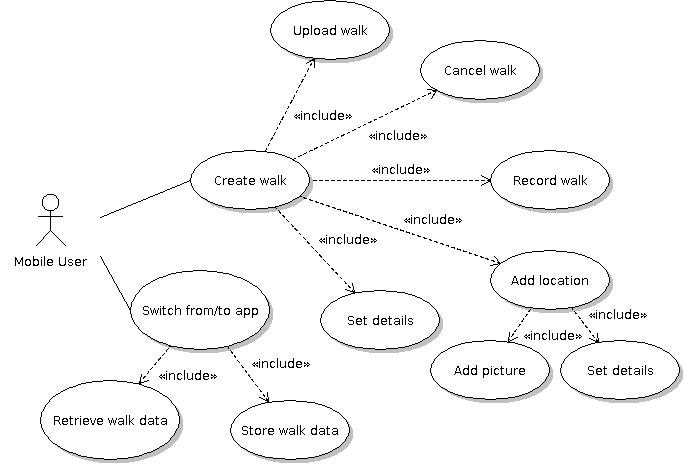
\includegraphics[width=1\linewidth]{AppUseCase}
    }
\end{figure}

\newpage

The app's use cases include: 

\subsubsection{Create Walk (FR1)}
Here the user starts to create a walk. Once this interaction is started 
(by pressing the button in the app's main menu), and a valid walk name is provided, 
the user's location is tracked and periodically added to the on-going walk's list of GPS points.\newline
As a part of this case the user may choose to: 

\begin{itemize}
\item Add location: This will allow the user to add the current location to the walk as a point of interest. (FR3)
		\begin{itemize}
		\item Take picture: The user can take a picture to add to this location. (FR4)
		\item Set details: The user can set the location's details (name, description).
		\end{itemize}
\item Set details: The user can set the walk's details (title, short decription(<100 characters), long description(<1000 characters). (FR2)
\item Cancel walk: The user may choose at any point to cancel their walk. This will stop recording their position and drop all current data of the on-going walk. (FR5)
\end{itemize}

\subsubsection{Upload Walk (FR6)}
This is used at the end of the "create walk" case in order to upload the walk to the server.

\subsubsection{Switch to/from app}
Whenever the user switches from the WTC app to another app, it will store the current walk's data. When they switch back it will retrieve the previously stored data. (FR7)

\subsection{Server}
\begin{figure}[H]
    \makebox[\linewidth]{
        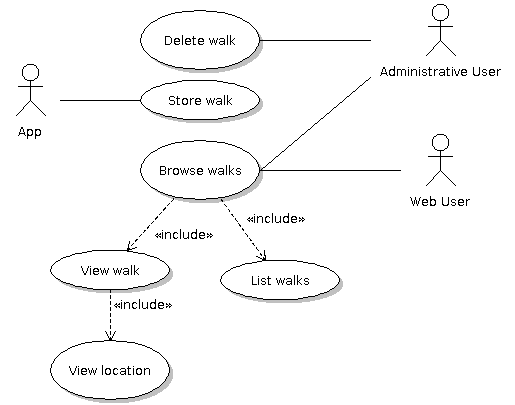
\includegraphics[width=1\linewidth]{ServerUseCase}
    }
\end{figure}

The server's use cases include several actors. \newline
The "App" actor is an instance of the WTC app on a client's phone and can upload walks. \newline
The "
User" is a client accessing the WTC website in a web browser. 
They may view a list of walks, select one, and view its details.\newline
The "Administrative User" is a user with the power to delete walks as well as view them.\newline
\bigskip

The server's use cases include: 

\subsubsection{Store walk}
A walk recieved from a client using the WTC app can be stored in the database of walks. . (FR9)

\subsubsection{Delete walk}
This use case allows for administrative users to delete any walks which they feel do not belong in the database.
This would include any corrupted/broken walks and walks which contain obscene or offensive content. 
 
\subsubsection{Browse walks}
This use case provides html pages to users which contains a list of all the walks in the database. The cases in this case are: 

\begin{itemize}
\item List walks: This provides a list of all the stored walks.
\item View walk: This will allow the user to view a specific walk, including its name, short and long descriptions, and its points of interest. (FR8)
		\begin{itemize}
		\item View location: This will allow a user to look at a specific point of interest. This includes its name, description, location, and any picture it has.
		\end{itemize}
\end{itemize}

\section{USER INTERFACE DESIGN}

\subsection{Android Application UI Design}
This section of the documentation will give an idea for how the UI of both the Android application and the web application
will look like and also the flow of the program from screen to screen. These designs are not final due to technical
restraints we may face later on in development but they will give a feel for the sort of layout and feel we are working towards.

\subsubsection{Main Menu (FR1)}
\bigskip
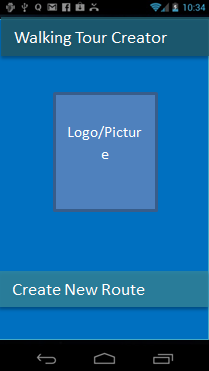
\includegraphics{PhoneUI1}
\bigskip

The first screen that the user is presented with is the main menu. This screen has one main option for the user to select.
The user can create a new route which allows them to progress into the application and start recording their routes.
There will also be some sort of logo or picture above these options.

\subsubsection{Create New Route (FR2)}
\bigskip
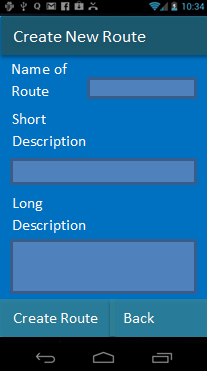
\includegraphics{PhoneUI2}
\bigskip

On the Create New Route screen the user is able to set up a new route for them to record.
They will be presented with a field to enter the name of the route, a short description
of the route and a longer description. The short description will be restricted to up to 
100 characters while the long description is up to 1000 characters. The user will be 
required to fill in all of the fields, as per the functional requirements. 

\bigskip
There will be two buttons at the bottom which allow the route to be created or to go back to the previous page. 

\subsubsection{Create Route (FR1, FR5, FR6)}
\bigskip
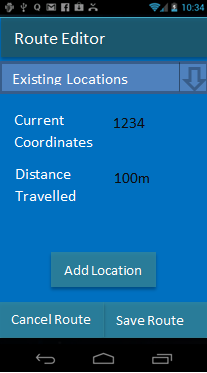
\includegraphics{PhoneUI3}
\bigskip

When the route has been created the user will be presented with their current coordinates which will update in real 
time as the user moves around, their current distance travelled from the starting location, along with options to 
add a location and save the current route.
\bigskip
The existing locations drop down will allow the editing of locations that have already been added, 
letting the user change the name, coordinates and description of a previous location.
\bigskip
Adding a location will save the current position and move to the next screen where they can specify information about that location.
Once the user has finished recording and has added their locations, the user can press the save location button at the bottom of the 
screen to send this data to the server where it can be read by the web application. They can also cancel the walk if they do not require it after recording.

\subsubsection{Adding Location (FR3, FR4, FR9)}
\bigskip
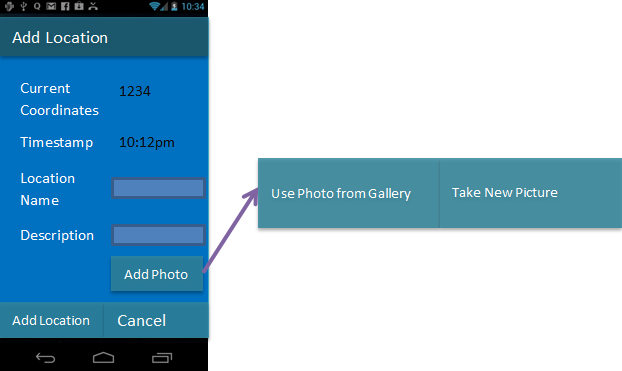
\includegraphics{PhoneUI4}
\bigskip

When adding the location the user is required to enter some information along with some already given to you.
The user?s current coordinates are displayed along with the current time the location was added.
The user then enters the name of the location and a short description.
There is also an option to add a photo where a photo can be taken using the camera option or use a photo already in the gallery.

\subsection{Web Application Design}
\subsubsection{HomePage}
\index{User interface design!Web Application Design!HomePage}
\begin{figure}[H]
    \makebox[\linewidth]{
        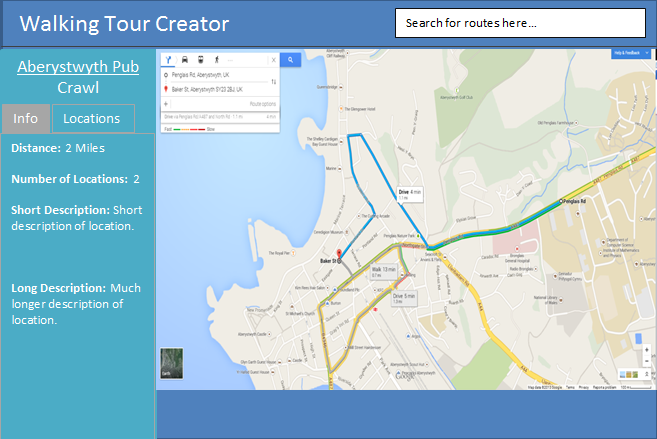
\includegraphics[width=1\linewidth]{WebUI1}
    }
\end{figure}
\bigskip
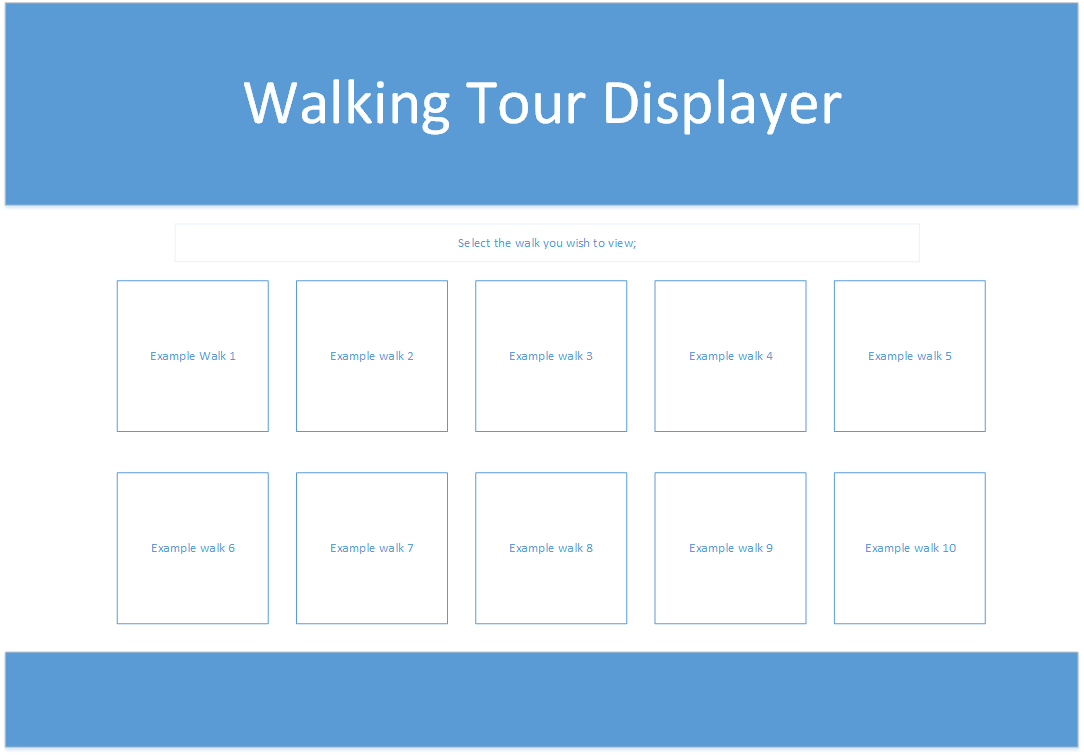
\includegraphics{WebUI2a}
\bigskip

There will be images on the home page of the walks. The user can then select a walk from the homepage. The user can then select this route which will then populate the sidebar and Google Map. 
The sidebar will allow the user to toggle between information about the walk and information about the locations, as there is not enough space to contain both.
\clearpage

\section{GANTT CHART}

\begin{figure}[H]
    \makebox[\linewidth]{
        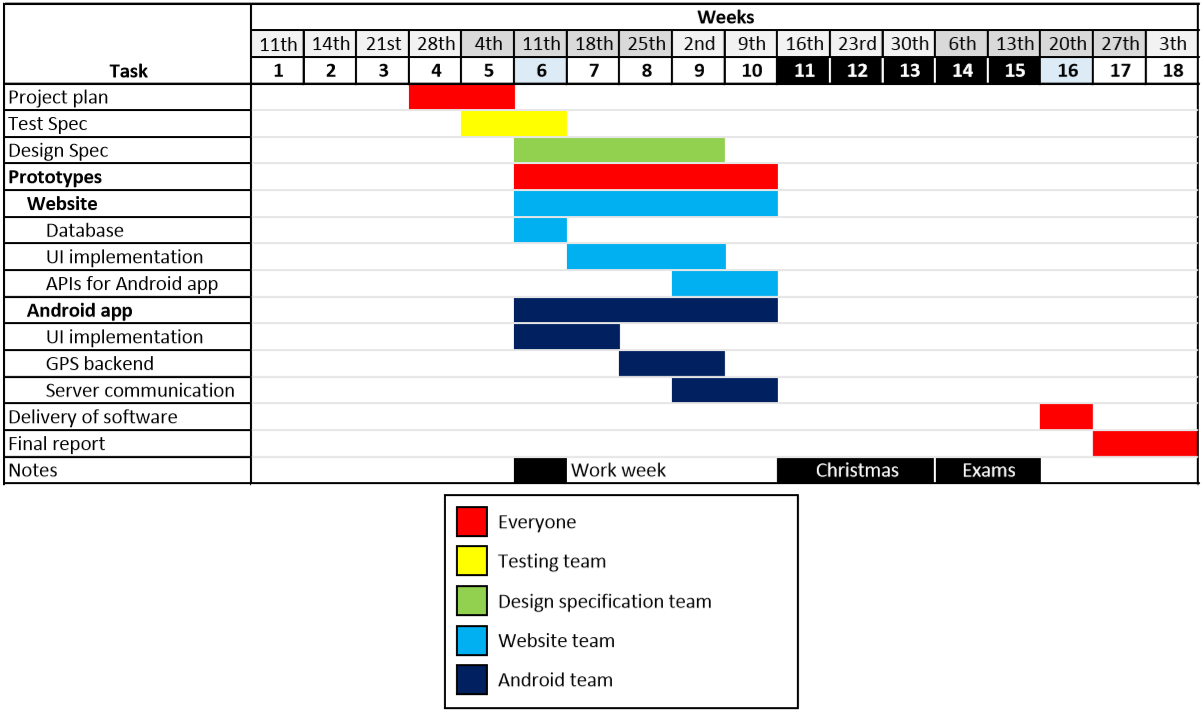
\includegraphics[angle=90,width=0.69\linewidth]{GanttChart}
    }
\end{figure}

\clearpage

\section{RISK ANALYSIS}
\subsection{Gold plating}
As programmers we sometimes like to show off our skills by adding unnecessary features to our program.
The schema clearly states that there are no extra marks for extra features and so doing this would just
be a waste of programming hours. This can be avoided by having a clear plan of what is needed for the
program before the actual programming starts.

\subsection{Illnesses}
This is an unavoidable risk. It is inevitable that members of the group will fall ill at some point during the year. 
To stop this becoming a problem, any members that fall ill will need to let the group know as soon a possible, so that 
other members can help out with any work that the ill member had been assigned. It is then the responsibility of the 
ill member of the group to then put in some extra work time when he recovers from illness. Also more than one programmer will work on and understand each part of the code.

\subsection{Time management}
One of the biggest risks for the group is that we will run out of time and that the project will be unfinished in the due date,
or that all members of the group will have to start putting in crazy hours, in a desperate attempt to get the program done.
Again this can be avoided by having a clear plan, where each specific part of the website and program have a clear completion deadline.
 
\subsection{Compromising on design}
In order to get stuck into the harder tasks of a program earlier, programmers will compromise on design on the easier parts of the program. This is also a waste of programming hours as design is arguably the most important part of a program.
 
\subsection{Backups}
The worst situation that could happen is that all the data that the group has been working on gets lost. This is avoided by having multiple backups of our program,
and not just on the same hard drive. These backups need to be made in a separate physical location, and also need to be made every time work has been done on the project. As well as several physical copies, all the work will be constantly updated and stored on github.

\subsection{Released project has low quality}
There is always the risk that the project, when completed is of low quality. 
This can be avoided by assuring that everyone is happy with suggested Interface design and everyone is clear on what needs to be done. 
We will also need to ensure a disciplined development is used.

\subsection{Conflicting Ideas}
As programmers, we are all likely to have our own ideas on how we think the app should be developed. 
To avoid any conflict, any issues that an individual may have with the design of the app, 
will have to bring them forward sooner rather than later. This will overall make for a happy group who will be able to work efficiently as a team.



\newpage

\section{APPENDIX D: REVISED DESIGN SPECIFICATION}


\subsection{DECOMPOSITION DESCRIPTION}
\subsection{Programs in system}
The system is composed of two programs:
\begin{itemize}
\item The Walking Tour Creator Android application
\item The Walking Tour Displayer website
\end{itemize}


\subsubsection{Walking Tour Creator}
The Walking Tour Creator is an application to allow the user can create walks
on a mobile device for them to be uploaded to the server. It implements the
requirements (FR1), (FR2), (FR3), (FR4), (FR5), (FR6), (FR7), (FR9), (PR1) and
must conform with the requirements (EIR1), (PR2), (DC1), (DC2).\cite{se.qa.rs}

This application will use a GUI as a means for the user to create a walk. The
user will be able to walk around an area and the GPS component of their device
will capture the route that they take. Along the route, they can mark points of
interest, which contains a description and optionally a photo. Once the user
has completed the walk, they can choose to either discard their creation or
upload it to the Walking Tour Displayer.

\subsubsection{Walking Tour Displayer}
The Walking Tour Displayer is website for viewing walks created by users via
the Walking Tour Creator. It implements the requirements (FR8), (FR9), (PR1)
and must conform to the requirements (EIR1), (PR2), (DC1), (DC2),
(DC3).\cite{se.qa.rs}

The walks are stored in a MySQL database with the attributes specified in
(DC3). The database will be queried by the website and allow the user to select
a walk. The selected walk would then be displayed on a map, and the user can
select a points of interest along the route of the walk.

\newpage

\subsection{Significant classes in each program}
\subsubsection{Significant classes in Walking Tour Creator}
\emph{MainAppActivity}. This is the main class of the application.

\emph{WalkCreatorActivity}. This is an activity panel holding the UI for
recording the walk. It also has a Location Listener running in the backgorund recording the users walk

\emph{Walk}. This contains a list of the coordinates of the route that the user
is creating, and the metadata of the walk.

\emph{PointOfInterest}. This contains a point of interest in the route, which
is a coordinate with a description and optionally a photo of what is in that.

\subsubsection{Significant functions in Walking Tour Displayer}
\emph{intialize}. This JavaScript function creates an embedded Google Map on
the page.

\emph{addMarker}. This JavaScript function takes coordinates as parameters and
sets a marker on the map using them.

\emph{addPath}. This JavaScript function takes two coordinates as parameters
and it sets a path on the map using them.


\subsection{Mapping requirements onto classes}
\begin{tabular}{|l |l |}
\hline
\emph{Requirement} & \emph{Classes providing requirement} \\
\hline
FR1 & MainAppActivity \\
\hline
FR2 & WalkCreatorActivity, Walk \\
\hline
FR3 & WalkCreatorActivity, Walk, PointOfInterest  \\
\hline
FR4 & WalkCreatorActivity \\
\hline
FR5 & WalkCreatorActivity \\
\hline
FR6 & WalkCreatorActivity \\
\hline
FR7 & MainAppActivity \\
\hline
FR8 & N/A \\
\hline
FR9 & WalkCreatorActivity \\
\hline
\end{tabular}


\newpage


\subsubsection{DEPENDENCY DESCRIPTION}
\subsubsection{Component Diagrams}

\subsubsection{Component Diagram for Walking Tour Creator}
\begin{figure}[h] 

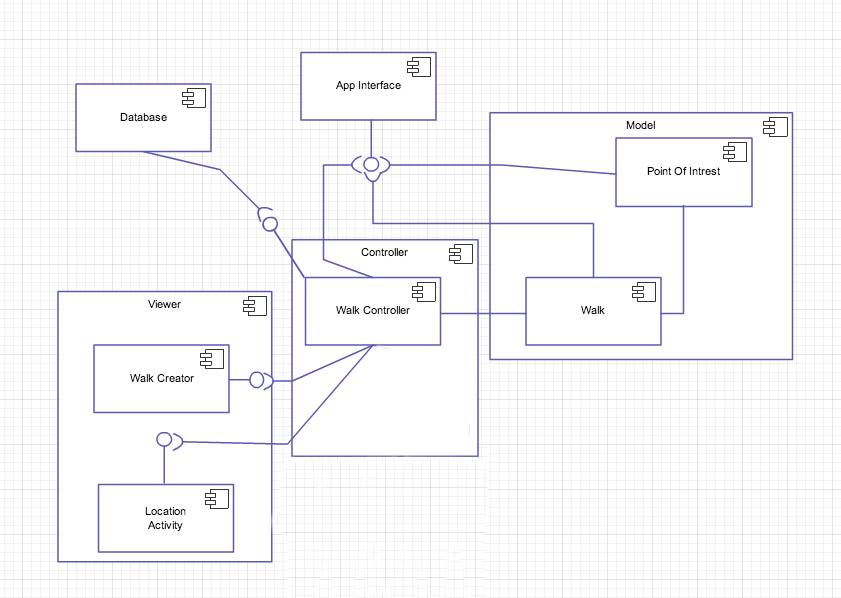
\includegraphics[width=15cm]{NewComponentDiagram.jpg}
\end{figure}

\newpage

\subsubsection{Component Diagram for Walking Tour Displayer}
\begin{figure}[h] 
    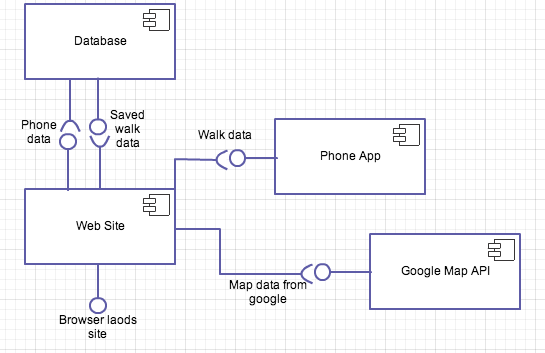
\includegraphics[width=15cm]{compontent_diagram_WTD.png}
\end{figure}

\newpage

\subsubsection{Inheritance Relationships}
The class with the most dependency is the WalkController, which has GPS
recording, walk creator and location activity. Just about all of the classes
need WalkController and this is where the app will send the data from the walk
made from the app to the website. Walk has a dependency with PointOfInterest
because it calls the gets and sets from that class. WalkCreatorActivity does GPS recording passes to controller then to walk. WalkCreatorActivity has the most dependancies.

For basic understanding of the dependencies of the Walking Tour Creator:
\begin{itemize}
\item Walk controller on walk creator and Location activity.
\item Walk on point of interest and walk controller.
\item Web site on walk controller.
\end{itemize}

The website has dependancies on the database to be able to get data of the
walks and to be able display them on the map and also show the description of
the walk on the side panel next to the map. Finally, the phone has a dependency
on the website because the data from the walk needs to go though the website to
be able to send the data to the database.      

For basic understanding of the dependencies of the Walking Tour Creator:
\begin{itemize}
\item Website on database and Google Maps API.
\item Phone app on website. 
\end{itemize}

\newpage

\subsection{INTERFACE DESCRIPTION}
\subsubsection{MainAppActivity interface specification}
\begin{verbatim}/**
 * This activity is shown when the user opens the app.
 * It has a single button which allows the user to "Create a walk". 
 * This button launches the "WalkDetailsActivity" Activity.
 *
 * @author Group 14
 */
public class WalkDetailsActivity {
   /**
    * This is the method which launches the "WalkCreatorActivity" Activity.
    * This is called when the user presses the "Create route" button.
    */
   public void createWalk();
}\end{verbatim}

\subsubsection{WalkDetailsActivity interface specification}
\begin{verbatim}/**
 /*
 * @(#) IPointOfInterest.java 1.0 2014-01-31
 *
 *
 */


/**
 * This interface is used represent a point of interest.
 * This will store a String name, String description,
 * Location object, and optional String representing
 * a picture associated with the point
 * @author Group14
 *
 */
public interface IPointOfInterest extends Parcelable {
   
   /**
    * This method is used to set the IPointOfInterest's name
    * @param name String representing the new name of the IPointOfInterest
    */
   public void setName(String name);
   
   /**
    * This method is used to get the IPointOfInterest's name
    * @return String representing the name of the IPointOfInterest
    */
   public String getName();
   
   /**
    * This method is used to set the IPointOfInterest's description
    * @param desc String representing the new description of the IPointOfInterest
    */
   void setDescription(String desc);
   
   /**
    * This method is used to get the IPointOfInterest's description
    * @return String representing the IPointOfInterest's description
    */
   public String getDescription();
   
   /**
    * This method is used to set the picture of the IPointOfInterest.
    * This must be a valid path to a picture in the filesystem.
    * @param picture String representing the location of the picture in the filesystem
    */
   public void addPicture(String picture);
   
   /**
    * This method is used to get the picture of the IPointOfInterest
    * @return A string representing the location on the filesystem of the picture
    */
   public String getPicture();
   
   /**
    * This method is used to get the IPointOfInterest's latitude
    * @return A double representing the IPointOfInterest's latitude
    */
   public double getLatitude();
   
   /**
    * This method is used to get the IPointOfInterest's longitude
    * @return A double representing the IPointOfInterest's longitude
    */
   public double getLongitude();
   
   /**
    * This method is used to get the IPointOfInterest's timestamp.
    * @return long timestamp in the unix epoch format.
    */
   public long getTime();
   
   /**
    * This method is used to get the IPointOfInterest's Location object
    * @return A Location object, representing the GPS location of the IPointOfInterest
    */
   public android.location.Location getLocation();
   
}
}
/*
 * @(#) IJsonPackager.java 1.0 2014-01-31
 *
 * Copyright (c) 2014 Aberystwyth University.
 * All rights reserved.
 *
 */
package uk.ac.aber.group14.model;

/**
 * This interface is used to convert an IWalk to a JSON String
 * @author Group14
 *
 */
public interface IJsonPackager {
   
   /**
    * This takes an IWalk and converts it into a JSON String
    * @param w The walk which will be converted
    * @return A String containing the walk represented as a JSON object
    */
   public String JSONify(IWalk w);
   
}
\end{verbatim}

\newpage


\subsubsection{Walk interface specification}
\begin{verbatim}/**
 /*
 * @(#) IWalk.java 1.0 2014-01-31
 *
 *
 */
package uk.ac.aber.group14.model;


/**
 * This interface is used to represent a walk
 * This stores a collection of Location objects,
 * a collection of IPointOfInterest objects,
 * a String name, String short description, and String
 * long description.
 * @author Group14
 *
 */
public interface IWalk extends Parcelable{

   /**
    * This method is used to add a single IPointOfInterest to the IWalk
    * @param point The point to add to the IWalk
    */
   public void addPointOfInterest(IPointOfInterest point);
   
   /**
    * This method is used to add a LinkedList of Location objects to the IWalk
    * @param locations The Locations to add to the IWalk
    */
   public void addLocations(java.util.LinkedList<android.location.Location> locations);
   
   /**
    * This method is used to set the name of the IWalk
    * @param name String representing the name of the walk
    */
   public void setName(String name);
   
   /**
    * This method is used to set the short description of the IWalk
    * @param desc String representing the short description of the IWalk
    */
   public void setShortDescription(String desc);
   
   /**
    * This method is used to set the long description of the IWalk
    * @param desc String representing the long description of the IWalk
    */
   public void setLongDescription(String desc);
   
   /**
    * This method is used to return the points of interest
    * as an array of PointOfInterest
    * @return An array of type PointOfInterest representing all the points of interest in the IWalk
    */
   public IPointOfInterest[] getPointsOfInterest();
   
   /**
    * This method is used to return the GPS locations as an array of
    * type Location
    * @return An array of type Location representing all of the Locations in the IWalk
    */
   public android.location.Location[] getLocations();
   
   /**
    * This method is used to get the name of the IWalk
    * @return A String representing the name of the IWalk
    */
   public String getName();
   
   /**
    * This method is used to get the short description of the IWalk
    * @return A String representing the short description of the IWalk
    */
   public String getShortDescription();
   
   /**
    * This method is used to get the long description of the IWalk
    * @return A String representing the long description of the IWalk
    */
   public String getLongDescription();
   
   /**
    * This method is used to add a single Location to the IWalk
    * @param location The Location to add to the walk
    */
   public void addLocation(Location location);
   
   /**
    * This method is used to get the number of Location objects
    * in the IWalk
    * @return An int representing the number of Location objects in the IWalk
    */
   public int getNumberLocations();
   
   /**
    * This method is used to get the number of IPointOfInterest objects
    * in the IWalk
    * @return An int representing the number of IPointOfInterest objects in the IWalk
    */
   public int getNumberPOI();
}

\end{verbatim}

\newpage

\subsection{DETAILED DESIGN}
\subsubsection{Sequence diagrams}

\begin{figure}[h] 

   
\includegraphics[width=15cm]{New_Sequence_Diagram_Group_Project_14.png}
    
\end{figure}

\newpage

\subsubsection{Significant algorithms}
\textbf{SetMarkers}
SetMarkers basically takes points from the database and plots them using the LineBetweenPoints function and the google API. It takes in the latitude and longitude from a 2 dimensional array and plots the points on the map

\textbf{LineBetweenPoints}
LineBetweenPoints uses the google API to go from of marker to the next and plots a route in between them. Before we discovered the API,we thought to write our own version in java. 
see the JSon document for the data transmission algorithms.


\subsubsection{Significant data structures}
The data structures we will be using are the IPointOfInterest interface and the
IWalk interface.

The IWalk interface will be implemented by a class and will hold all of the
points of interest. It is the current plan to use a LinkedList due to it being
dynamic in size. If the team member implementing the interface has a compelling
enough reason to use an alternative means of storing them then they can do. Due
to it being an interface this will be up to whoever implements it - the public
methods will remain the same.

The IPointOfInterest will be used to store the data about a point of interest.
For storing the pictures it is again likely that a LinkedList will be used.

The Location objects will be stored in a LinkedList in the walk
whilst they are being recorded. This will allow us to quickly and easily add
new Location objects to the end of it. Unlike an array, we will not need to
repeatedly recreate the list with a larger amount of memory each time a new
location is added.


\clearpage

\addcontentsline{toc}{section}{REFERENCES}
\begin{thebibliography}{5}
\bibitem{se.qa.03} \emph{Software Engineering Group Projects}
General Documentation Standards.
C. J. Price, N. W. Hardy, SE.QA.03. 1.5 Release.
\bibitem{se.14.design} \emph{Software Engineering Group Projects}
Design Specification.
Group 14, SE.14.DESIGN. 1.2 Release.
\end{thebibliography}
\addcontentsline{toc}{section}{DOCUMENT HISTORY}
\section*{DOCUMENT HISTORY}
\begin{tabular}{|l | l | l | l | l |}
\hline
Version & CCF No. & Date & Changes made to Document & Changed by \\
\hline
0.1 & N/A & 2014-02-09 & Initial creation with performance reports & jmt14 \\
\hline
0.2 & N/A & 2014-02-14 & Management summary draft & tht5 \\
\hline
0.3 & N/A & 2014-02-14 & Critical evaluation & jam64 \\
\hline
0.4 & N/A & 2014-02-14 & Final state of the project & rab26 \\
\hline
0.5 & N/A & 2014-02-14 & Historical account of the project & jam66 \\
\hline
0.6 & N/A & 2014-02-14 & Maintenance manual initial draft & rab26, jab73 \\
\hline
0.7 & N/A & 2014-02-14 & Minor changes to language to meet QA & jmt14 \\

\hline
\end{tabular}
\label{thelastpage}
\end{document}
